\subsection{Jet Classification}
{{\footnotesize
\noindent This benchmark evaluates ML models for real-time classification of
particle jets using high-level features derived from simulated LHC data. It
includes both full-precision and quantized models optimized for FPGA deployment.


\begin{description}[labelwidth=4cm, labelsep=1em, leftmargin=4cm, itemsep=0.1em, parsep=0em]
  \item[date:] 2024-05-01
  \item[version:] v0.2.0
  \item[last\_updated:] 2024-05
  \item[expired:] unknown
  \item[valid:] yes
  \item[valid\_date:] 2024-05-01
  \item[url:] \href{https://github.com/fastmachinelearning/fastml-science/tree/main/jet-classify}{https://github.com/fastmachinelearning/fastml-science/tree/main/jet-classify}
  \item[doi:] 10.48550/arXiv.2207.07958
  \item[domain:] Particle Physics
  \item[focus:] Real-time classification of particle jets using HL-LHC simulation features
  \item[keywords:]
    - classification
    - real-time ML
    - jet tagging
    - QKeras
  \item[licensing:] Apache License 2.0
  \item[task\_types:]
    - Classification
  \item[ai\_capability\_measured:]
    - Real-time inference
    - model compression performance
  \item[metrics:]
    - Accuracy
    - AUC
  \item[models:]
    - Keras DNN
    - QKeras quantized DNN
  \item[ml\_motif:]
    - Real-time
  \item[type:] Benchmark
  \item[ml\_task:]
    - Supervised Learning
  \item[solutions:] Solution details are described in the referenced paper or repository.
  \item[notes:] Includes both float and quantized models using QKeras

  \item[contact.name:] Jules Muhizi
  \item[contact.email:] unknown
  \item[datasets.links.name:] JetClass
  \item[datasets.links.url:] \href{https://zenodo.org/record/6619768}{https://zenodo.org/record/6619768}
  \item[results.links.name:] ChatGPT LLM
  \item[results.links.url:] \href{https://docs.google.com/document/d/1runrcij-eoH3\_lgGZ8wm2z1YbL1Qf5cSNbVbHyWFDs4}{https://docs.google.com/document/d/1runrcij-eoH3\_lgGZ8wm2z1YbL1Qf5cSNbVbHyWFDs4}
  \item[fair.reproducible:] True
  \item[fair.benchmark\_ready:] True
  \item[id:] jet\_classification
  \item[Citations:] \cite{duarte2022fastml}
\end{description}

{\bf Ratings:} ~ \\

\begin{tabular}{p{0.15\textwidth} p{0.07\textwidth} p{0.7\textwidth}}
\hline
Rating & Value & Reason \\
\hline
dataset & 5 & None
 \\
documentation & 4 & Full reproducibility requires manual setup
 \\
metrics & 5 & None
 \\
reference\_solution & 4 & HW/SW requirements missing; Reference not bundled as official starter kit
 \\
software & 3 & Not containerized; Setup automation/documentation could be improved
 \\
specification & 4 & System constraints missing
 \\
\hline
\end{tabular}

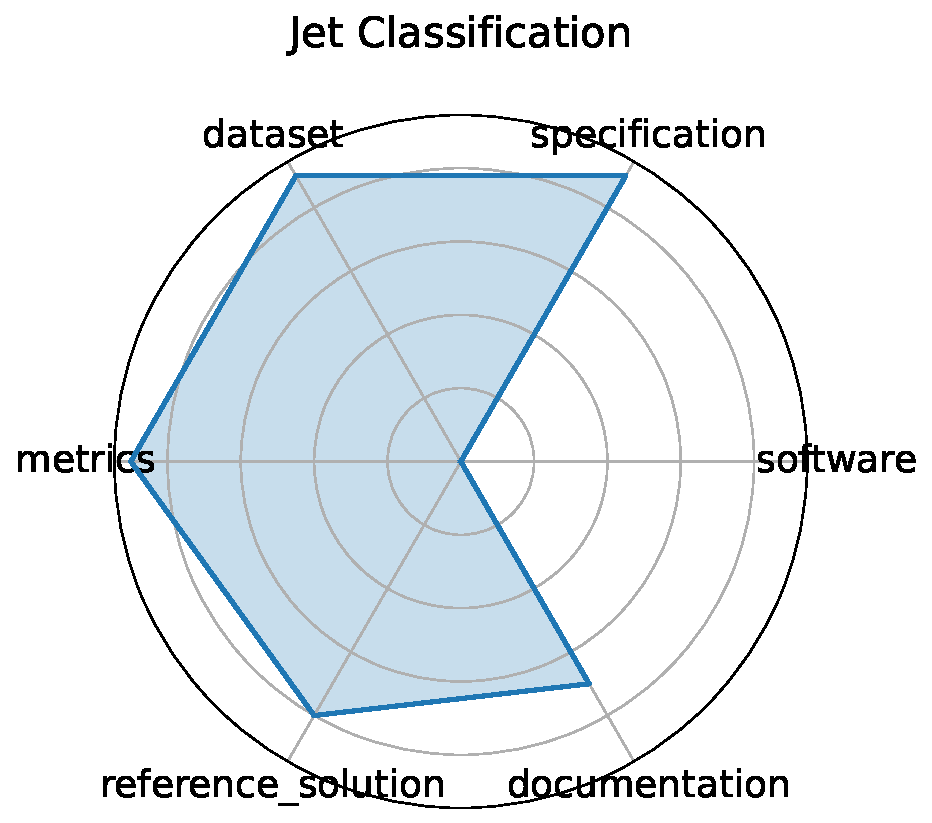
\includegraphics[width=0.2\textwidth]{jet_classification_radar.pdf}
}}
\clearpage